The IMU communicates with the Arduino via the I2C bus. This must be implemented in the Simulink design. The sensor values obtained from this must now be further ground via Matlab function blocks. To get more trustworthy data in the later course of the program, a Kalman filter was also used. However, this filter needs both the measured angle and the measured yaw rate for proper operation. Therefore these two values were calculated. 

\begin{figure}[H]
    \centering
    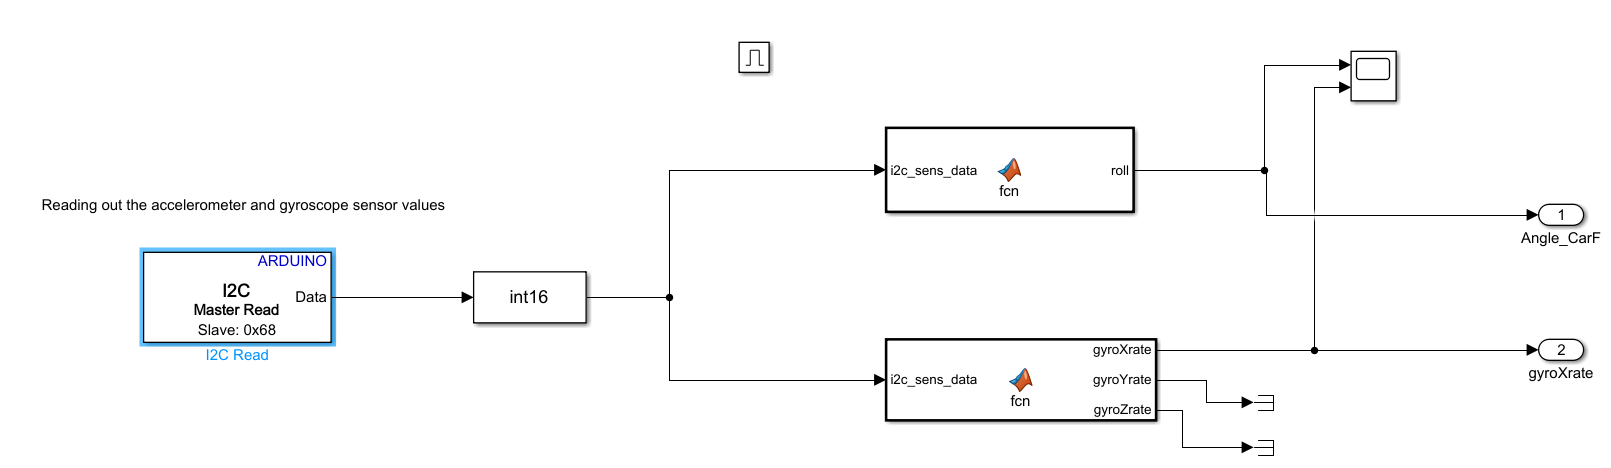
\includegraphics[width=\textwidth]{Lab_report/pics/hardware_impl/gyro_read.PNG}
    \caption{data reading Submodel}
    \label{fig:acc_gyro_read}
\end{figure}

\begin{lstlisting}[language=Matlab, caption=angle calculation]
function roll = fcn(i2c_sens_data)
    accX = double(i2c_sens_data(1));
    accY = double(i2c_sens_data(2));
    accZ = double(i2c_sens_data(3));
    roll = atan(accY / sqrt(accX * accX + accZ * accZ)) * 180/pi; 
end
\end{lstlisting}

\begin{lstlisting}[language=Matlab, caption=gyro rate calculation]
function [gyroXrate,gyroYrate,gyroZrate] = fcn(i2c_sens_data)
    gyroX = double(i2c_sens_data(5));
    gyroY = double(i2c_sens_data(6));
    gyroZ = double(i2c_sens_data(7));
    gyroXrate = gyroX/131;
    gyroYrate = gyroY/131;
    gyroZrate = gyroZ/131; 
end
\end{lstlisting}